\documentclass[12pt, oneside]{article}
\usepackage[letterpaper, margin=1in, headsep=0.5in, left=0.3in, right=2.5in]{geometry}
\usepackage[english]{babel}
\usepackage[utf8]{inputenc}
\usepackage{amsmath}
\usepackage{amsfonts}
\usepackage{amssymb}
\usepackage{tikz}
\usepackage{yhmath}
\usetikzlibrary{quotes, angles}
\usepackage{graphicx}
\usepackage{enumitem}
\usepackage{multicol}

\newif\ifmeta
\metatrue %print standards and topics tags

\title{Regents Geometry}
\author{Chris Huson}
\date{April 2022}

\usepackage{fancyhdr}
\pagestyle{fancy}
\fancyhf{}
\renewcommand{\headrulewidth}{0pt} % disable the underline of the header
\raggedbottom

%\fancyhead[LE]{\thepage}
\fancyhead[RO]{Name:}
\fancyhead[LO]{BECA / Dr. Huson / Geometry Regents Mixed Review}
\cfoot{\thepage}

\begin{document}
\subsubsection*{11.5 Circle equations and chords}
\begin{enumerate}[itemsep=2cm]
\item What are the coordinates of the center and the length of the radius of the circle whose equation is $(x+3)^2+(y-7)^2=4$?
  
\item What is the equation of a circle with diameter $\overline{AB}$ with $A(2,-1)$, $B(8,7)$?
    \begin{flushright}
      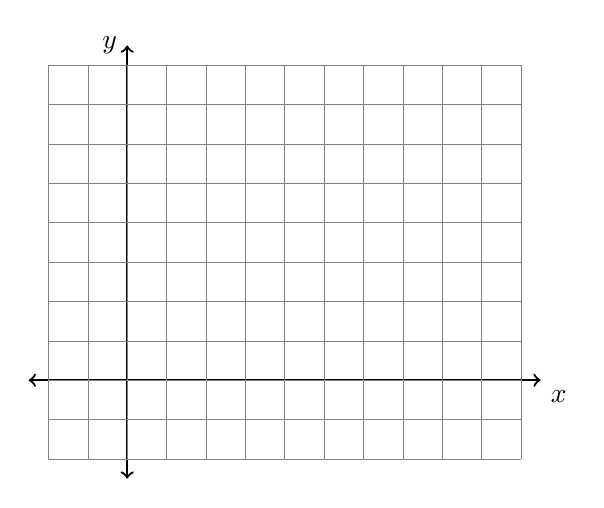
\begin{tikzpicture}[scale=0.5]
        \draw [thick, <->] (-2.5,0) -- (10.5,0) node [below right] {$x$};
        \draw [thick, <->] (0,-2.5)--(0,8.5) node [left] {$y$};
        \draw [help lines] (-2,-2) grid (10,8);
          %\draw (5,3) circle[radius=5];
          %\fill (5,3) circle[radius=.1]node[right]{$O$};
          %\draw (2,-1) --(8,7);
      \end{tikzpicture}
    \end{flushright}

\item %January 2018
The equation of a cirle is $x^2+y^2-6x+2y=6$. What are the coordinates of the center and the length of the radius of the circle? \vspace{2cm}
%  \begin{enumerate}
%    \item center $(-3,1)$ and radius 4
%    \item center $(3,-1)$ and radius 4
%    \item center $(-3,1)$ and radius 16
%    \item center $(3,-1)$ and radius 16
%  \end{enumerate}
    

\item Circle $O$ has chords $\overline{AD}$ and $\overline{BE}$ intersecting at $C$, as shown. Find $BC$.\\
  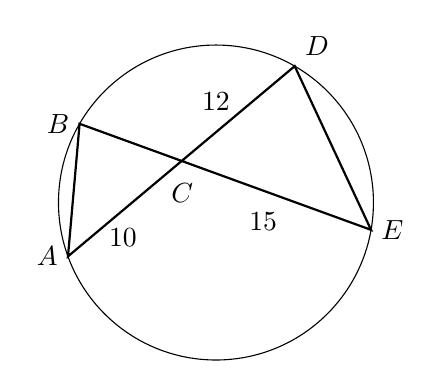
\begin{tikzpicture}[scale=0.4]
   \draw (0,0) circle[radius=5];
   \draw [thick]
   (-10:5) node[right] {$E$}--
   (150:5) node[left] {$B$}--
   (200:5) node[left] {$A$}--
   (60:5) node[above right] {$D$}--cycle;
   \draw (140:1.4) node[below] {$C$};
   \draw (90:3.8) node[below] {$12$};
   \draw (190:3) node[below] {$10$};
   \draw (0:1.5) node[below] {$15$};
  \end{tikzpicture}


\newpage
\item An isosceles right triangle whose legs measure 6 is continuously rotated about one of its legs to form a three-dimensional object. The three-dimensional object is a
  \begin{enumerate}
    \item cylinder with a diameter of 6
    \item cylinder with a diameter of 12
    \item cone with a diameter of 6
    \item cone with a diameter of 12
  \end{enumerate}

\item The coordinates of the endpoints of directed line segment $ABC$ are $A(-8,7)$ and $C(7,-13)$. If $AB:BC = 3:2$, what are the coordinates of $B$?

\item A circle with a diameter of 10 cm and a central angle of $30^\circ$ is drawn below.
\begin{center}
  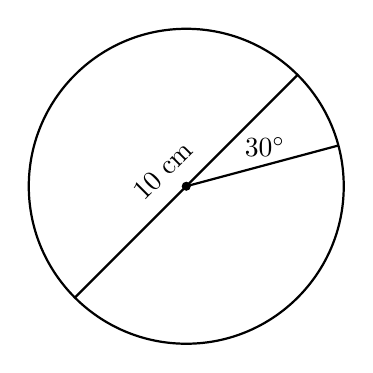
\begin{tikzpicture}[scale=1, rotate=0]
    \draw [thick] (45:2)--(225:2);
    \draw [thick] (0,0)--(15:2);
    \draw [fill] (0,0) circle [radius=0.05];
    \draw [thick](0,0) circle [radius=2];
    \node at (1,0.5){$30^\circ$};
    \node at (-0.3,0.2)[rotate=45]{$10 \; \rm{cm}$};
  \end{tikzpicture}
  \end{center}
  What is the area, to the \emph{nearest tenth of a square centimeter}, of the sector formed by the $30^\circ$ angle?

\item A child's tent can be modeled as a pyramid with a square base whose sides measure 60 inches and whose height measures 84 inches. What
is the volume of the tent, to the \emph{nearest cubic foot}?

\end{enumerate}
\end{document}
  